\documentclass[12pt]{article}
\usepackage[english]{babel}
\usepackage[utf8x]{inputenc}
\usepackage{amsmath}
\usepackage{graphicx}
\usepackage[a4paper]{geometry}
\usepackage{multirow}
\usepackage{lscape}
\usepackage{multirow}
\usepackage{float}

\begin{document}
\begin{titlepage}

% definition of custom command for horizontal lines
\newcommand{\HRule}{\rule{\linewidth}{0.5mm}}

\center
% HEADING
\textsc{\LARGE University of Dublin,\\Trinity College}\\[1.0cm]

\includegraphics[width=0.2\textwidth]{logo.png}

\HRule \\[0.4cm]
\textsc{\Large League Table Investigation}\\[0.25cm]
\textsc{\large ST2004 \& ST2353 Assessment 2}\\[0.1cm]
\HRule \\[0.4cm]
 
% AUTHORS
\begin{minipage}{0.5\textwidth}
\begin{flushleft} \large
\emph{Authors:}
\\Alexandru \textsc{Sulea} 12315152
\\Edmond \textsc{O'Flynn} 12304742
\\Jonathan \textsc{Lester} 14310385
\\Ronan \textsc{Campbell} 14324880
\end{flushleft}
\end{minipage}
~
\begin{minipage}{0.4\textwidth}
\begin{flushleft} 
\large
\emph{Lecturer:} \\
Dr. Brett \textsc{Houlding}
\vspace{1.9cm}
\end{flushleft}
\end{minipage}\\[2cm]

% DATE
{\large \today}\\[1cm] 

% LOGO

\includegraphics[width=0.3\textwidth]{ball.jpeg}
\clearpage
\end{titlepage}

\tableofcontents
\addcontentsline{toc}{section}{References}
\thispagestyle{empty}
\cleardoublepage
\setcounter{page}{1}
\pagebreak

\newgeometry{top=1cm,left=1cm,bottom=2cm,right=1cm}
\section{Q1i: Monte Carlo Simulation of Equal Skill}
\clearpage
\section{Q1ii: Monte Carlo Simulation of Unequal Skill}
\subsection{Validation of Simulation}
The simulation was modified such that there is now an array of skills where the Monte Carlo simulation is now of unequal skill between teams. The probabilities are randomly generated via the \emph{RAND()} function, and this skill coefficient remains constant throughout the season as a measure between 0 and 1.

\begin{table}[h]
\centering
\begin{tabular}{ccccc}
\multirow{2}{*}{\begin{tabular}[c]{@{}c@{}}Ability\\ Scores\end{tabular}} & A & B    & C    & D   \\
                                                                          & 1 & 0.91 & 0.19 & 0.1
\end{tabular}
\caption{Unequal Ability Scores for 4 Teams}
\end{table}

The frequency of points gained by each team depends highly on the given abilities of the teams. Teams with equal abilities tend to gain equal quantities of points within the stochastic process. Teams of differing abilities illustrates a trend of higher or lower cumulative probabilities of point-gaining as shown in the plots. A simulation of 1000 repetitions was performed on the system, resulting in the following frequencies:

\begin{table}[h]
\centering
\begin{tabular}{ccccc}
     & A & B & C & D \\
1    & 6 & 4 & 2 & 0 \\
2    & 5 & 5 & 2 & 1 \\
3    & 4 & 4 & 3 & 2 \\
4    & 6 & 5 & 2 & 2 \\
1000 & 4 & 5 & 2 & 1
\end{tabular}
\caption{Point Frequency per Rep}
\end{table}

It is important to note that teams \emph{A} and \emph{B}, with their given higher abilities, demonstrate a much higher frequency of wins throughout the league, which both validates and pertains to the given expectation of the stochastic system.

\begin{figure}[h]
\centering
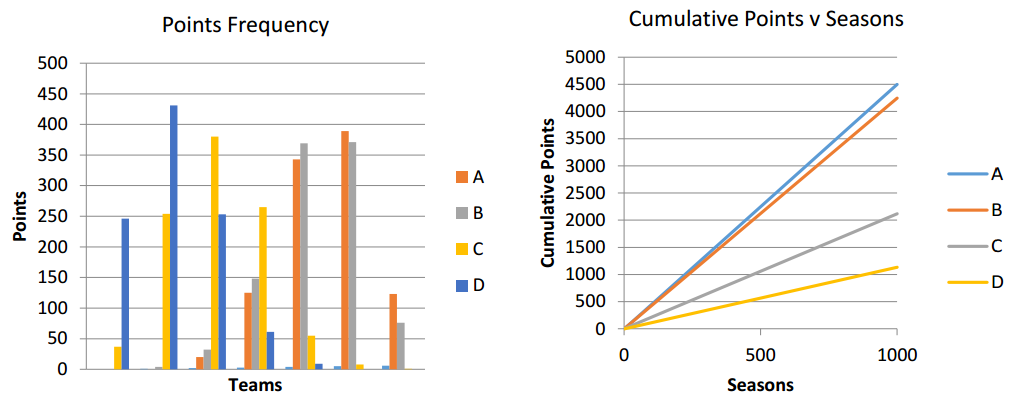
\includegraphics[width=0.6\textwidth]{q1ii_graphs.png}
\caption{Distributions of Points v Frequency}
\end{figure}

\subsection{Probability Distributions}
Within the scope of when all teams except A having equal skills is true, the number of wins within the league is demonstrated accordingly on the plots. In the simulation of the league, the number of wins were sampled using the following characteristic equation $A_{skill}$ vs $n \cdot B_{skill}$, where $n$ is sampled at $0.5$, $1$, and $2$. Empirically, these demonstrate ranges of wins using the given skill coefficients in order to simulate "half as skilled", "equally skilled", and "twice as skilled".

\begin{figure}[H]
\centering
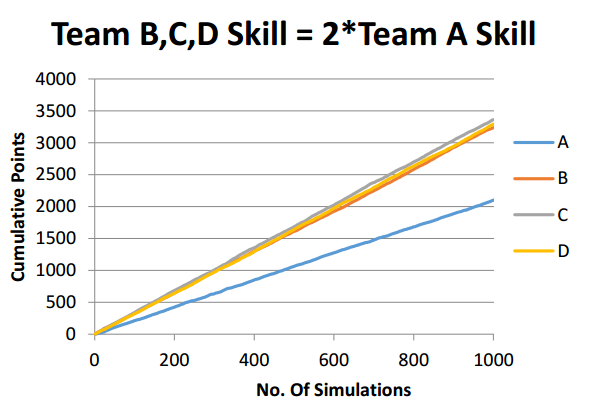
\includegraphics[width=0.4\textwidth]{twice_skill_a.png}
\caption{Distributions of Inter-Team Skill}
\end{figure}

From the graphs in figures x and x, the number of wins is a representation of the effect of skill within the league, thus reinforcing the results obtained.

\begin{figure}[h]
\centering
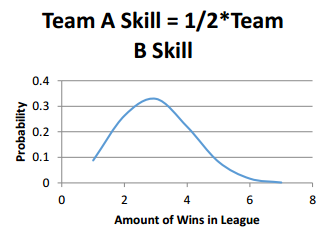
\includegraphics[width=0.25\textwidth]{skill_a_half_skill_b.png}
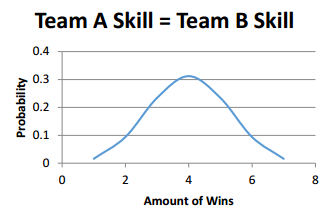
\includegraphics[width=0.25\textwidth]{skill_a_equals_skill_b.png}
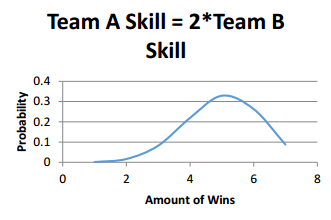
\includegraphics[width=0.25\textwidth]{skill_a_2x_skill_b.png}
\caption{Distributions of Inter-Team Skill}
\end{figure}

\section{Q1iii: Various Skills within a Group of Ten}
In order to investigate the argument that the variation in the skills of the different teams positively affects the variation across the teams in the number of matches won, simulations for skill ranges of 1-10, 1-100 and 1-1000 were run. Each team was assigned a letter ranging from A-J and each team was given a random skill rating. In order to account for home advantage I opted to give each side a skill bonus of “x”\% where “x” is a randomly assigned value between 1 and 100. This is to account for the fact that home advantage doesn’t affect all teams the same.

\begin{table}[h]
\centering
\begin{tabular}{cccccccccccc}
          & A    & B    & C    & D    & E     & F   & G    & H    & I    & J    & SD Skill \\
Skill     & 5    & 1    & 3    & 9    & 6     & 7   & 4    & 3    & 5    & 2    & 2.415    \\
Home Adv. & 32   & 75   & 47   & 70   & 97    & 100 & 74   & 27   & 73   & 1    &          \\
At Home   & 6.55 & 1.75 & 4.41 & 15.3 & 11.82 & 14  & 6.96 & 3.81 & 8.65 & 2.02 &         
\end{tabular}
\caption{Random Skill Levels for Each Team Between 1-10}
\end{table}

“p” was assigned to the probability of the home team R of skill level “a”, defeating away team S of skill level “b”. A call to \emph{RAND()} was made to obtain the results of the games. If RAND()\textless p, then the home team R wins, else the away team S wins, where given $h=1+\frac{x}{100}$, $$p=\frac{ha}{ha+b}$$ 

\begin{table}[h]
\centering
\begin{tabular}{ccccccccccccc}
H-A   & A     & B     & C     & D     & E     & F     & G     & H     & I     & J     &  &          \\
A     &       & 0.868 & 0.686 & 0.421 & 0.522 & 0.483 & 0.621 & 0.686 & 0.567 & 0.766 &  &          \\
B     & 0.259 &       & 0.368 & 0.163 & 0.226 & 0.200 & 0.304 & 0.368 & 0.259 & 0.467 &  &          \\
C     & 0.469 & 0.815 &       & 0.329 & 0.424 & 0.387 & 0.524 & 0.595 & 0.469 & 0.688 &  &          \\
D     & 0.764 & 0.939 & 0.836 &       & 0.718 & 0.686 & 0.793 & 0.836 & 0.754 & 0.884 &  &          \\
E     & 0.703 & 0.922 & 0.798 & 0.568 &       & 0.628 & 0.747 & 0.798 & 0.703 & 0.855 &  &          \\
F     & 0.737 & 0.933 & 0.824 & 0.609 & 0.700 &       & 0.778 & 0.824 & 0.737 & 0.875 &  &          \\
G     & 0.582 & 0.874 & 0.699 & 0.436 & 0.537 & 0.499 &       & 0.699 & 0.582 & 0.777 &  &          \\
H     & 0.432 & 0.792 & 0.559 & 0.297 & 0.388 & 0.352 & 0.488 &       & 0.432 & 0.656 &  &          \\
I     & 0.634 & 0.896 & 0.742 & 0.490 & 0.59  & 0.553 & 0.684 & 0.742 &       & 0.812 &  &          \\
J     & 0.288 & 0.699 & 0.402 & 0.183 & 0.252 & 0.224 & 0.336 & 0.402 & 0.288 &       &  &          \\
      &       &       &       &       &       &       &       &       &       &       &  &          \\
H-A   & A     & B     & C     & D     & E     & F     & G     & H     & I     & J     &  &          \\
A     &       & A     & A     & D     & E     & F     & A     & A     & I     & J     &  &          \\
B     & A     &       & C     & D     & E     & F     & G     & H     & I     & B     &  &          \\
C     & A     & C     &       & D     & C     & C     & G     & H     & C     & J     &  &          \\
D     & D     & D     & C     &       & D     & F     & D     & D     & D     & D     &  &          \\
E     & E     & E     & C     & E     &       & E     & G     & E     & E     & E     &  &          \\
F     & A     & F     & F     & F     & F     &       & F     & F     & F     & F     &  &          \\
G     & G     & B     & C     & D     & G     & F     &       & G     & I     & G     &  &          \\
H     & H     & H     & H     & H     & H     & F     & H     &       & I     & H     &  &          \\
I     & I     & I     & I     & D     & I     & F     & G     & I     &       & J     &  &          \\
J     & A     & J     & J     & J     & J     & F     & G     & H     & I     &       &  &          \\
      &       &       &       &       &       &       &       &       &       &       &  & SD Score \\
Score & 8     & 2     & 8     & 12    & 9     & 15    & 9     & 10    & 10    & 7     &  & 3.367   
\end{tabular}
\caption{Simulation of 1 Season}
\end{table}

A season comprised of 90 games in total, each team played a home leg and an away leg against every other team. At the end of the season the total number of wins for each side was added up and called the score. As visible from Fig.1, Fig.3 and Fig.4, the standard deviation of both the skill level and score was calculated and recorded. In order to obtain reliable results, a total of 2000 seasons were simulated. Data was then taken and used to plot a graph of skill standard deviation vs score standard deviation.
\begin{table}[h]
\centering
\begin{tabular}{ccc}
     & Skill Deviation & Score Deviation \\
1    & 229.491         & 2.582           \\
2    & 174.076         & 3.266           \\
3    & 193.196         & 2.494           \\
4    & 267.227         & 4.269           \\
1000 & 337.221         & 3.742          
\end{tabular}
\caption{Skill Deviation vs Score Deviation over 1000 Reps}
\end{table}
One would expect there to be a greater variation in the score given a greater variation in the skill. Across 2000 seasons with the skill ranged from 1-100 and an average skill standard deviation of approximately 28.6, the average of the score standard deviation was approximately 3.69. When the skill rating ranged from 1-1000 with an average standard deviation of around 286, the average score standard deviation was roughly 3.76. For a smaller skill rating range of 1-10 with small skill standard deviation of around 2.83, the score standard deviation was around 3.41. Using the \emph{Law of Large Numbers}, we can conclude that the mean of the standard deviations calculated after 2000 simulations are somewhat close to the expected value for the standard deviations of score and skill. There is a slight increase in the standard deviation of the score when the skill range is increased. Obviously the increase in the score standard deviation is unlikely to be dramatic because each team only plays 18 matches. The R2 value for each graph implies a limited correlation between the standard deviation in the skill and in the score.
\\\\
A 95\% confidence interval for each standard deviation was calculated and determined, and found that the average standard deviation for infinitely many seasons for the skill range of 1-1000 lies in the interval ($3.75 \pm 0.046$), for a skill range of 1-100 it lies in the interval ($3.73 \pm 0.045$) and for a skill range of 1-10 it lies in the interval ($3.41 \pm 0.041$). From this we can see that the intervals for the skill ranges of 1-1000 and 1-100 overlap however the difference between skill ranges of 1-10 and both 1-100 and 1-1000 are statistically significant.
\\\\
When Fig.5, Fig.6 and Fig7 are compared, generally there is an increase in the standard deviation of the score, this implies that the variation in skill does have an effect on the variation of the score, however it is also evident that the effect of the skill variation is limited between the skill ranges of 1-100 and 1-1000. What can be drawn from this extrapolation is that when the skill variation is very small, a smaller score variation exists than in a league with a large skill variation, however the score variation between two leagues of large and very large skill variations should still yield a similar score variation.
\clearpage
\section{Q2: Kelly Betting}
\subsection{Kelly Criterion}
The Kelly Criterion is a formula which is used to maximize profit when betting on a on an event with a positive Expected Value. It was devised in 1956 by John L. Kelly Jnr. after whom the criterion is named. The criterion advises the gambler on the optimal percentage of their bankroll to bet based on the probability of winning and the odds provided on the wager. This percentage will provide the highest returns in the long run however this comes with a high level of volatility, so much so that many supporters of the Kelly Criterion encourage utilizing a fraction of the percentage the criterion advises you to bet.
\\
Kelly criterion is as follows
$$f=\frac{bp-q}{b}=\frac{p(b+1)-1}{b}$$
where given the following
\begin{align*}
f&=\text{fraction of bankroll to wager}\\
b&=\text{net odds received on wager}\\
p&=\text{probability of winning}\\
q&=\text{probability of loss}=1-p
\end{align*}

For even-money bets, the formula can be simplified further to
$$f=2p-1$$
As we can see from the formula, when the probability of a loss is greater than the net odds times the probability of a win we find a negative value for the bankroll fraction. This means the bettor should take the opposite position on the bet. However, this is not always possible as we can see in casino games such as roulette. In European Roulette when betting on red or black, the Kelly Criterion gives us a value of -0.027. This value tells us to bet on our chosen colour \emph{not} coming up. Unfortunately the casino does not offer this bet and therefore the Kelly bettor cannot employ his strategy at this game. This is one of the large drawbacks of the Kelly Criterion.

\subsection{Simulation}
A simulation was carried out in Excel to investigate the supposed benefits of the Kelly Criterion. Using the \emph{RAND()} function, a random number was generated and this decided the outcome of the bet. Firstly Kelly betting was compared to flat stake betting and then fractional Kelly betting was compared to find why many supporters advise using a fraction of the percentage that the Kelly Criterion would tell us to wager. A running bankroll of each strategy was kept and the simulation was run 1000 times.
\subsection{Discussion}
From the simulation, we can see that in the long run, utilizing the Kelly Criterion maximizes our potential bankroll. Relative to betting with a flat stake, Kelly betting is far more profitable but this was only apparent after a large number of bets. In fact, in the short term, flat betting was a far more stable strategy albeit slower to profit. From the graph produced, Kelly betting is clearly highly volatile however as the number of trials increases, the returns from Kelly betting are astronomical.

\begin{figure}[H]
\centering
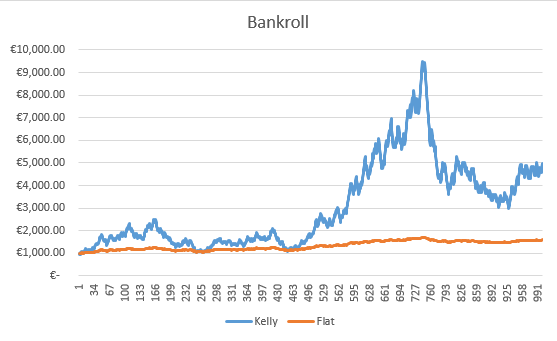
\includegraphics[width=0.5\textwidth]{kelly_flat.PNG}
\caption{Cumulative Bankroll}
\end{figure}

The second simulation examined the effects of using a fraction of the advised Kelly percentage on the long term returns and the volatility of the strategy. Betting greater multiples of the Kelly percentage sees the gambler receive huge returns in the long run however the gambler significantly increases his risk of ruin as we see increased volatility. However, betting lesser multiples of the Kelly percentage sees lower, more stable returns but they are still above the levels of that of a flat bettor. This highlights the reason many people advise using a more conservative version of the Kelly Criterion for the casual bettor and even the investor, it decreases the volatility while still seeing a good share of the increased profit that the full Kelly Criterion can provide.

\begin{figure}[H]
\centering
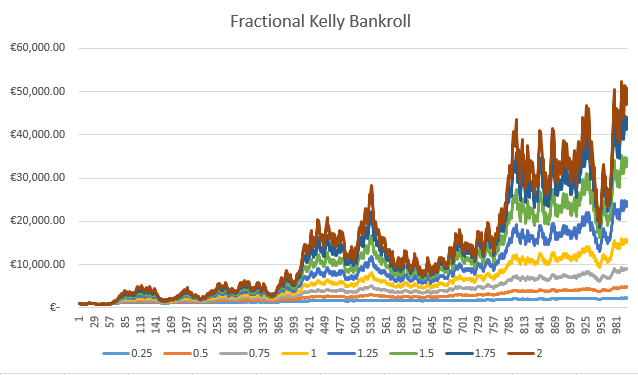
\includegraphics[width=0.5\textwidth]{frac_kelly.PNG}
\caption{Fractional Kelly Bankroll}
\end{figure}

Another reason for using a more conservative percentage is that Kelly betting is almost always utilized in a scenario where the bettor has to estimate the true odds of an event rather than calculating them e.g. result in a football match rather than a casino game. This is due to the fact that games where the exact odds of winning are easily calculated, the casino or bookmaker offering the bet will always provide odds less than that of the actual probability of a win to ensure they make profit in the long term. Therefore we cannot use the Kelly Criterion in these situations, we must look for possible bets where we feel the bookmaker has priced the bet wrong and we think that the event has a higher chance of happening than the bookmaker does. In this case we can use the Kelly Criterion as this bet, we believe, holds a positive expected value. Unfortunately many gamblers overestimate their odds of winning and this can cause an inflated Kelly percentage. Combining the inflated Kelly percentage with the high volatility of high Kelly percentages will often cause the gambler to run into ruin. Betting less than the Kelly percentage corrects for this.
\subsection{Conclusion}
The benefits of the Kelly Criterion can also be taken advantage of in investing in the stock market, however this requires a large amount of estimation and as such, a lesser fraction of the Kelly percentage should be used in these situations also.
\\\\
The Kelly Criterion provides gamblers and investors with a method of maximizing their profit when presented with a favourable betting or investing opportunity. However this comes at the price of high volatility and the need for a large amount of trials, therefore a more conservative fraction of the Kelly percentage should be used to avail of the increased profitability and reduce volatility along with risk of ruin.
\begin{thebibliography}{3}
\bibitem{kilbyj}
  Jim Kilby, Jim Fox, Anthony F. Lucas,
  \emph{Casino Operation Management, 2nd Edition},
  Wiley (2006).
\end{thebibliography}
\end{document}
